% Drawing 138/07-12 -- folder 138, batch 07, archive page 130 (PDF page 131).
% Transcription: une sphère découpée en fuseaux par des méridiens joignant deux pôles (« orange »).
% Kind: sphere cut into lunes (« orange »). Method 2 (schematic redraw from the facsimile). Status: ok.
% Notes: A sphere cut into lunes by meridians joining two poles (« orange »): the outline and three visible meridians.
% Coordinates: 1 unit = 1 mm = 1/100 of the crop width (bbox in page fractions: [0.14, 0.122, 0.34, 0.215]).
% Redrawn by Claude (claude-opus-5-5), issue #73, 2026-11-07; not checked by a human; not compiled (no TeX in the session).
% Rights: reproduces part of the work -- behind RENDER_TRANSCRIPTS, never published by itself.
\documentclass[tikz,border=3pt]{standalone}
\usepackage{amsmath,amssymb}
\usetikzlibrary{patterns,arrows.meta}
\tikzset{pencil/.style={black!45}, struck/.style={black!35}, mark/.style={circle,draw,inner sep=1.3pt}, pt/.style={circle,fill,inner sep=0.9pt}, opt/.style={circle,draw,fill=white,inner sep=1.1pt}}
\begin{document}
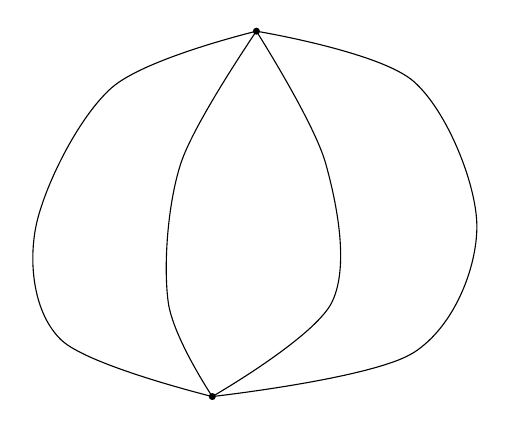
\begin{tikzpicture}[x=1mm,y=1mm,line cap=round,line join=round,font=\scriptsize]
\draw plot[smooth, tension=0.55] coordinates {(60,-7.6) (41.6,-14.8) (32,-32.4) (35.2,-46.8) (54.4,-54)};
\draw plot[smooth, tension=0.55] coordinates {(60,-7.6) (80,-14) (88,-32.4) (80,-48.4) (54.4,-54)};
\draw plot[smooth, tension=0.55] coordinates {(60,-7.6) (50.4,-24.4) (48.8,-42) (54.4,-54)};
\draw plot[smooth, tension=0.55] coordinates {(60,-7.6) (68.8,-24.4) (69.6,-42) (54.4,-54)};
\node[pt] at (60,-7.6) {};
\node[pt] at (54.4,-54) {};
\end{tikzpicture}
\end{document}
